\subsection{Tool-Use Optimization}


\begin{table*}[!t]
\centering
\caption{
Representative \textbf{Tool-Use Optimization} systems categorized by \textit{Integration Stage}, \textit{Learning Type}, and \textit{Tool Strategy}. 
}
\renewcommand{\arraystretch}{1.15}
\setlength{\tabcolsep}{6pt}
\begin{tabular}{p{3cm}>{\centering\arraybackslash}p{3cm}>{\centering\arraybackslash}p{4cm}>{\centering\arraybackslash}p{5.5cm}}
\toprule
\textbf{Method} & \textbf{Stage} & \textbf{Learning} & \textbf{Tool Strategy} \\
\midrule
\rowcolor[HTML]{F5F5F5}
\multicolumn{4}{l}{\textbf{Modality I: In-Context Integration}} \\
ReAct~\cite{yao2023react} & Inference & Prompting & Interleaved reasoning–action \\
ART~\cite{paranjape2023artautomaticmultistepreasoning} & Inference & Few-shot & Retrieved multi-step demos \\
ChatCoT~\cite{chen-etal-2023-chatcot} & Inference & Prompting & CoT with tool calls \\
GEAR~\cite{lu-etal-2024-gear} & Inference & Delegation & Light model for tool selection \\
AVATAR~\cite{NEURIPS2024_2db8ce96} & Inference & Contrastive & In-context tool reasoning \\
\midrule
\rowcolor[HTML]{F5F5F5}
\multicolumn{4}{l}{\textbf{Modality II: Post-Training Integration}} \\
Toolformer~\cite{schick2023toolformer} & Post-train & Self-sup. + SFT & Self-generated API calls \\
ToolLLM~\cite{DBLP:conf/iclr/QinLYZYLLCTQZHT24} & Post-train & SFT & Large-scale API demos \\
ToolAlpaca~\cite{DBLP:journals/corr/abs-2306-05301} & Post-train & SFT & Simulated dialogues \\
ReSearch~\cite{chen2025learning} & Post-train & RL + Reflec. & Adaptive retrieval reasoning \\
ReTool~\cite{dong2025reinforcement} & Post-train & RL & Reinforced code execution \\
ToolRL~\cite{qian2025toolrl} & Post-train & RL & Multi-tool policy learning \\
\midrule
\rowcolor[HTML]{F5F5F5}
\multicolumn{4}{l}{\textbf{Modality III: Orchestration-based Integration}} \\
HuggingGPT~\cite{shen2023hugginggpt} & System & Planner–Exec. & Multi-tool coordination \\
TaskMatrix.AI~\cite{DBLP:journals/corr/abs-2303-16434} & System & Planner & Massive API ecosystem \\
ToolPlanner~\cite{liu2025toolplanner} & System & RL & Plan-before-act framework \\
OctoTools~\cite{lu2025octotoolsagenticframeworkextensible} & System & Rule-based & Hierarchical orchestration \\
ToolExpNet~\cite{DBLP:conf/acl/ZhangCZCDL25} & System & Embedding & Experience-based selection \\
ToolChain*~\cite{DBLP:conf/iclr/ZhuangC0MBRS024} & System & Search & A* decision over tools \\
\bottomrule
\end{tabular}
\label{tab:tool_use_methods}
\end{table*}

Tool use optimization is the capacity of an agent to augment its intrinsic capabilities by intelligently invoking external modules. This allows agents to overcome limitations such as outdated knowledge, inability to perform precise calculations, or lack of access to private information. The core challenge lies in the agent's ability to reason about \textbf{when} to use a tool, \textbf{which} tool to select from a library, and \textbf{how} to generate a valid call. In this section, we examine existing approaches to tool use optimization, which can be broadly classified into three styles: \textit{in-context tool-integration}, \textit{post-training tool-integration}, 
and \textit{orchestration-based tool-integration}.

% \ma{refine}
\subsubsection{In-Context Tool-integration} 


The in-context demonstration paradigm is a training-free approach to empowering LLMs with new capabilities at inference time. This method leverages the remarkable in-context learning ability of modern LLMs, guiding a frozen, off-the-shelf model to perform complex tasks by providing carefully crafted instructions, examples, and contextual information directly in the prompt.

% CoT based:
\paragraph{Interleaving Reasoning and Tool Use.}
The foundation of in-context agentic reasoning lies in augmenting the Chain-of-Thought (CoT) process with the ability to take action.\citep{wei2022chain}. 
{ChatCoT}~\cite{chen-etal-2023-chatcot} formalizes this paradigm by structuring reasoning traces as alternating "thought-tool-observation" steps in natural language, allowing LLMs to reflect on intermediate outputs and dynamically plan the next tool query.
While CoT enables LLMs to break down problems into intermediate reasoning steps, it operates in a closed world, limited by the model's internal knowledge. The key innovation in agentic tool use is to interleave these reasoning steps with actions (tool calls), creating a dynamic loop that allows the agent to interact with external environments to gather information and execute tasks \citep{inaba-etal-2023-multitool,trivedi2022interleaving}. 
ReAct \cite{yao2023react} introduced the "Reasoning+Acting" synergy. This approach enables the model to use reasoning to create, track, and adjust its action plans, while the actions allow it to interface with and gather information from external environments like knowledge bases or the web. 
Similarly, ART \cite{paranjape2023artautomaticmultistepreasoning} provides a structured approach by maintaining a library of successful task demonstrations. For a new task, ART retrieves a relevant multi-step exemplar and uses it as a few-shot prompt, guiding the LLM to follow a proven reasoning and tool-use path.



\paragraph{Optimizing Context for Tool Interaction.}
While the foundational interleaved loop is powerful, its performance degrades when agents must handle large or complex toolsets. A significant branch of research addresses this by optimizing the in-context information provided to the agent. Recent studies demonstrate that well-written tool documentation enables LLMs to utilize new tools in a zero-shot manner \citep{hsieh2023tooldocumentationenableszeroshot,yuan2024easytool}. This finding aligns with the key insight that LLMs, much like humans, benefit from clear and concise instructions. Alternatively, GEAR \citep{lu-etal-2024-gear} introduces a computationally efficient, training-free algorithm that delegates the tool selection process to a small language model while reserving the more powerful LLM for the final reasoning step to reduce costs.
AVATAR \cite{NEURIPS2024_2db8ce96} enhances the robustness of this choice by prompting the agent to perform in-context "contrastive reasoning" before acting.



While these in-context methods are flexible, their performance is ultimately bounded by the inherent capabilities of the frozen LLM and the length of its context window. 
Consequently, subsequent research has focused on post-training methods.

\begin{figure}
    \centering
    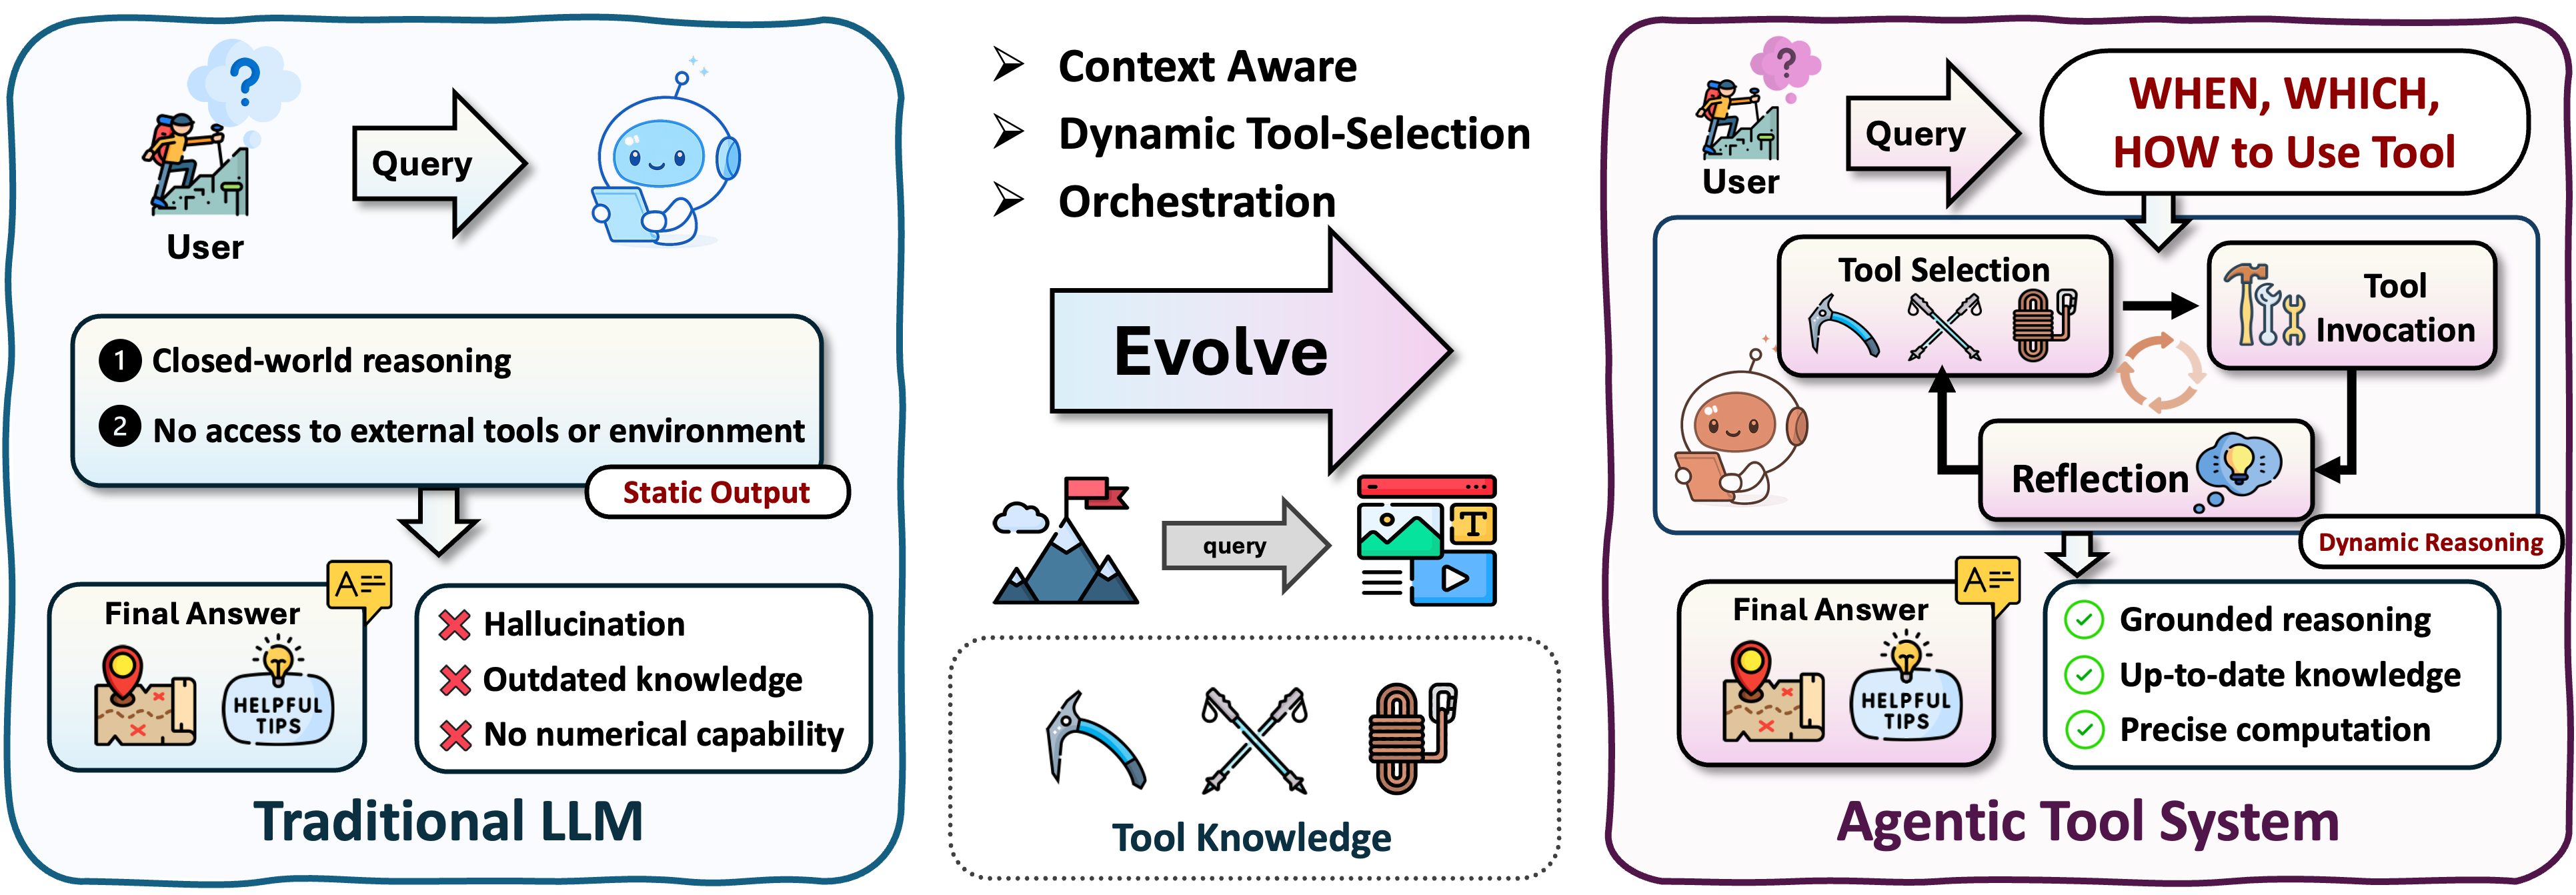
\includegraphics[width=\linewidth]{arxiv/figs/tool_use.png}
    \caption{Comparison between \textbf{traditional LLM} and \textbf{agentic tool-use} systems. While traditional models operate in a closed world with fixed reasoning, agentic tool-use systems enable dynamic selection, orchestration, and integration of external tools, allowing agents to extend reasoning, improve precision, and dynamically adapt across domains.}
    \label{fig:tool_use}
\end{figure}



\subsubsection{Post-training Tool-integration} Tool integration \citep{yao2023react, qu2025tool,shi2025tool} with post-training techniques has emerged as a key strategy for addressing the inherent limitations of LLMs or LRMs, such as outdated knowledge, limited computational precision, and shallow multi-step reasoning. By \textit{learning how to interact with external tools}, reasoning models can dynamically access up-to-date information, execute precise symbolic or numerical computations, and decompose complex tasks into grounded, tool-assisted reasoning steps \citep{wang2024empowering,yang2024buffer,singh2025agentic, cheng2024seeclick, zou2025reasonflux}. With tools as intermediaries, models are enriched and augmented by external capabilities, enabling the generation of more accurate and generalizable agentic reasoning trajectories \citep{nam2024using,yuan2024easytool,wu2025agentic}.

\paragraph{Bootstrapping of Tool Use via SFT.} \space Early works on tool-integration \citep{yao2023react, schick2023toolformer, DBLP:conf/iclr/QinLYZYLLCTQZHT24, DBLP:journals/corr/abs-2306-05301, lu2023chameleon, song2023restgpt, prasad2023adapt, yin2023agent, shi2024learning} primarily apply supervised fine-tuning (SFT) over curated tool-use reasoning steps, where models were trained to imitate demonstrations of search queries, code executions, or API calls. The SFT stage provided an initial competency in invoking tools, interpreting tool outputs, and integrating the results into coherent reasoning chains \citep{song2023restgpt, shinn2023reflexion}. For example, 
Toolformer \cite{schick2023toolformer} introduces a self-supervised framework in which large language models generate, validate, and retain useful API calls within unlabeled text, followed by fine-tuning on the filtered data to enhance factual accuracy and practical utility. 
ToolLLM \cite{DBLP:conf/iclr/QinLYZYLLCTQZHT24} further scales SFT training to over 16,000 real-world APIs, applying supervised fine-tuning on massive curated demonstrations to endow models with robust planning and invocation abilities. ToolAlpaca \cite{DBLP:journals/corr/abs-2306-05301} extends the idea to compact LLMs by automatically constructing a diverse toolset and generating multi-turn tool-use dialogues via multi-agent simulation, followed by fine-tuning to enable generalized tool-use even for previously unseen tools. While effective at bootstrapping tool-awareness, applying SFT along suffers from overfitting to the specific patterns in the training data \cite{kirk2023understanding, li2024preserving, o2024attributing, zou2025transformer}, leading to brittle tool-selection strategies and limited adaptability in unseen downstream application scenarios \citep{zeng2025itool,qian2025toolrl,yu2025demystifying}.

\paragraph{Mastery of Tool Use via RL.} \space Recent studies \citep{zhou2025sweet, qian2025toolrl, wei2025swe, chen2025learning, zhang2025rlvmr, jin2025search, zou2025autotool, dong2025reinforcement} leverages reinforcement learning (RL) during model post-training to go beyond imitation and achieve mastery in tool-integrated reasoning. With the integration of RL, models refine their tool-use strategies through outcome-driven rewards, learning \textit{when}, \textit{how}, and \textit{which} tools to invoke via trial and error \cite{chen2025learning, feng2025retool, dong2025reinforcement, sun2025zerosearch}. For instance, SWE-RL \citep{wei2025swe} optimizes code-editing policies on large-scale software evolution data, improving not only software issue resolution but also general reasoning skills. ReSearch \cite{chen2025learning} embeds search operations into multi-hop reasoning chains, enabling adaptive retrieval during complex QA. ReTool integrates real-time code execution into reasoning rollouts, leading to optimal performance on advanced math reasoning benchmarks. ToolRL \cite{qian2025toolrl} generalizes this paradigm to diverse toolsets by introducing principled reward designs for stable and scalable multi-tool learning. Across these settings, RL has been shown to yield more robust, adaptive, and generalizable tool-use policies than SFT alone, often transferring effectively to out-of-domain tasks \cite{team2025kimi1.5, comanici2025gemini, team2025kimi2, zeng2025glm, zou2025tattoo}.



\subsubsection{Orchestration-based Tool-integration} In real-world applications, tool use within complex systems often extends beyond the single-model, single-tool setting, requiring orchestration among multiple tools to complete complex tasks. This orchestration typically involves planning, sequencing, and managing dependencies across tools, i.e., ensuring that intermediate outputs are passed and transformed appropriately. Several early works \citep{shen2023hugginggpt, DBLP:journals/corr/abs-2303-16434, DBLP:conf/nips/HaoLWH23} explore this direction by devising strategies for the coordinated use of multiple tools, enabling systems to solve multi-stage tasks that no single tool can handle in isolation. Specifically, HuggingGPT \citep{shen2023hugginggpt} employs a centralized agent that leverages a language interface to plan which tools to invoke and when, enabling the solution of complex tasks requiring multiple tools in sequence. TaskMatrix.AI \citep{DBLP:journals/corr/abs-2303-16434} connects foundation models with millions of APIs, using the models to generate task-solution outlines and automatically matching certain sub-tasks to off-the-shelf models and systems with specialized functionalities. ToolkenGPT \citep{lu2025octotoolsagenticframeworkextensible} augments frozen language models with massive tool sets by encoding each tool as a special token during next-token prediction.

\paragraph{Agentic Pipelines for Tool Orchestration.} There are many frameworks designed to enable LLMs to call and orchestrate tools effectively. Most of the current agentic paradigm follows a “plan before action” strategy, where the model first generates a structured plan for tool use and then executes it. ToolPlanner \citep{liu2025toolplanner} introduces a two-stage reinforcement learning framework with path planning and feedback, supported by MGToolBench, to bridge the gap between API-heavy training data and real-world user instructions.
Tool-MVR \citep{DBLP:journals/corr/abs-2506-04625} enhances reliability and reflection through meta-verification of tool calls and exploration-based reflection learning, achieving strong gains over GPT-4 and other baselines.
More recently, 
OctoTools \citep{lu2025octotoolsagenticframeworkextensible} provides a training-free, extensible framework with standardized tool cards, a hierarchical planner, and an executor, showing broad improvements across multi-domain reasoning tasks.
Chain-of-Tools \citep{DBLP:journals/corr/abs-2503-16779} leverages frozen LLMs’ semantic representations to dynamically compose unseen tools in chain-of-thought reasoning, enabling generalization to massive tool pools without fine-tuning.
PyVision \cite{DBLP:journals/corr/abs-2507-07998} introduces an interactive, multi-turn framework that enables MLLMs to dynamically generate, execute, and refine Python-based tools, moving beyond static toolsets in visual reasoning. ConAgents \cite{shi2024learning} makes an initial extension of tool use frameworks for interactive multi-agent settings.
We are also glad to see emerging applications of such agentic tool orchestration frameworks in the chemistry domain \citep{DBLP:journals/corr/abs-2505-02484}.

\paragraph{Tool Representations for Orchestration.} Beyond designing orchestration pipelines, another line of research focuses on optimizing the tools themselves to facilitate more accurate selection, composition, and coordination during orchestration. ToolExpNet \citep{DBLP:conf/acl/ZhangCZCDL25} models tools and their usage experiences as a network that encodes semantic similarity and dependency relations, allowing LLMs to distinguish between similar tools and account for interdependencies during selection. 
T2Agent \citep{DBLP:journals/corr/abs-2505-19768} addresses multimodal misinformation detection by representing tools with standardized templates and using Bayesian optimization to select a task-relevant subset. Coupled with Monte Carlo Tree Search over this reduced action space, T2Agent enables efficient multi-source verification.
ToolChain* \citep{DBLP:conf/iclr/ZhuangC0MBRS024} frames the entire tool action space as a decision tree and applies A* search with task-specific cost functions to guide navigation. This representation allows efficient pruning of high-cost branches and identification of optimal tool-use paths.
ToolRerank \citep{DBLP:conf/coling/ZhengLLLLW24} refines tool retrieval by introducing adaptive truncation for seen vs. unseen tools and hierarchy-aware reranking to balance concentration (for single-tool queries) and diversity (for multi-tool queries).
